
	
	Как понять, что пользователю может понравиться товар? Первый вариант — поискать похожих на него пользователей и посмотреть, что нравится им; также можно поискать товары, похожие на те, которые этот пользователь уже покупал. Методы коллаборативной фильтрации строят рекомендации для пользователя на основе похожестей между пользователями и товарами, которые похожие пользователи выбирают.
	

	Существует два подхода к определению сходства между пользователями: Memory-based и Модель со скрытыми переменными
	
    Частью memory based является user-based. Его отличие от item-based и другие подробности про рекомендации смотрите здесь \url{https://github.com/hse-ds/iad-applied-ds/blob/master/2020/lectures/lecture01-recommender.pdf}
	
		
		\begin{figure}[H]
\centering
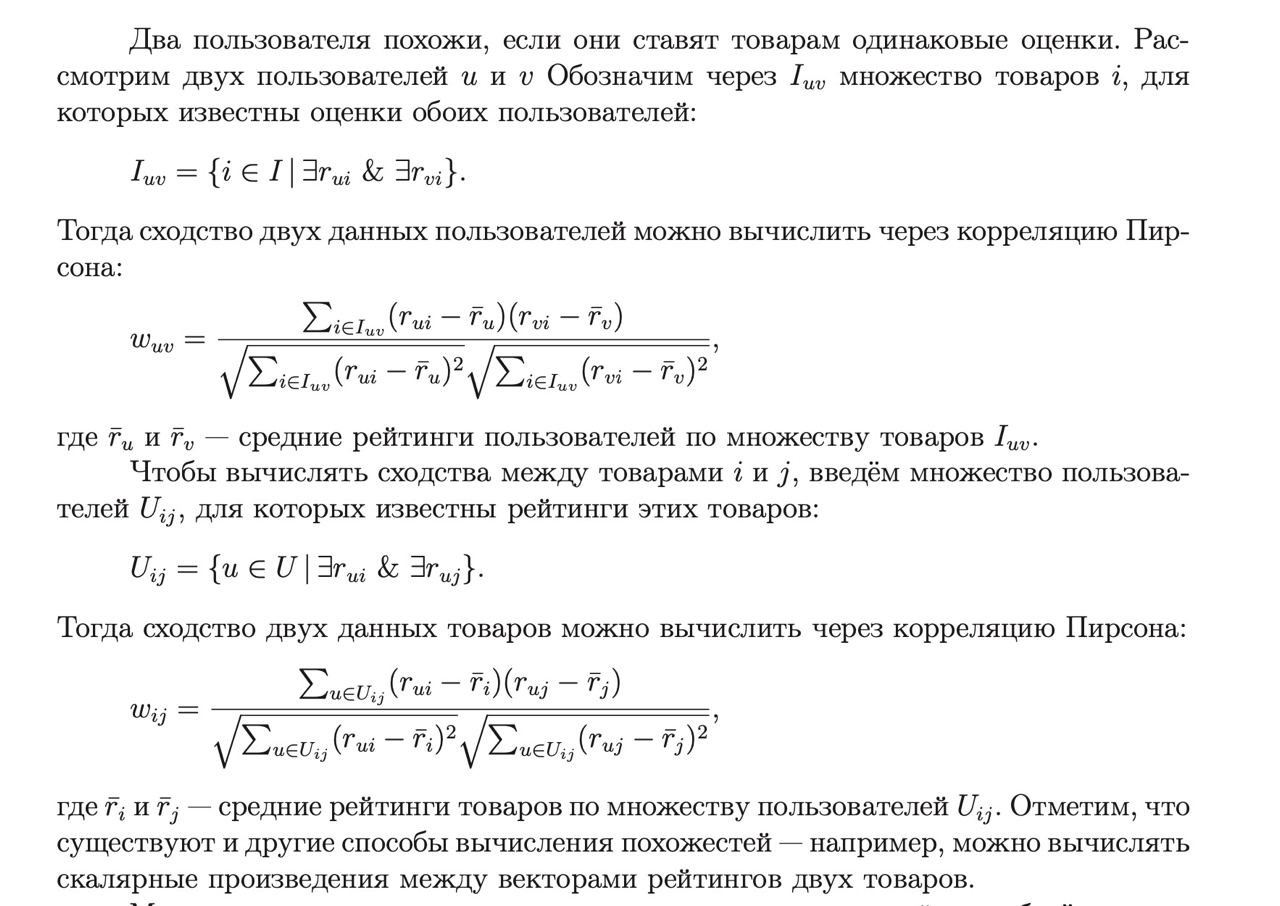
\includegraphics[width=0.7\linewidth]{16_memory1.jpg}
\label{fig:16_memory1} 
\end{figure}
	
			\begin{figure}[H]
\centering
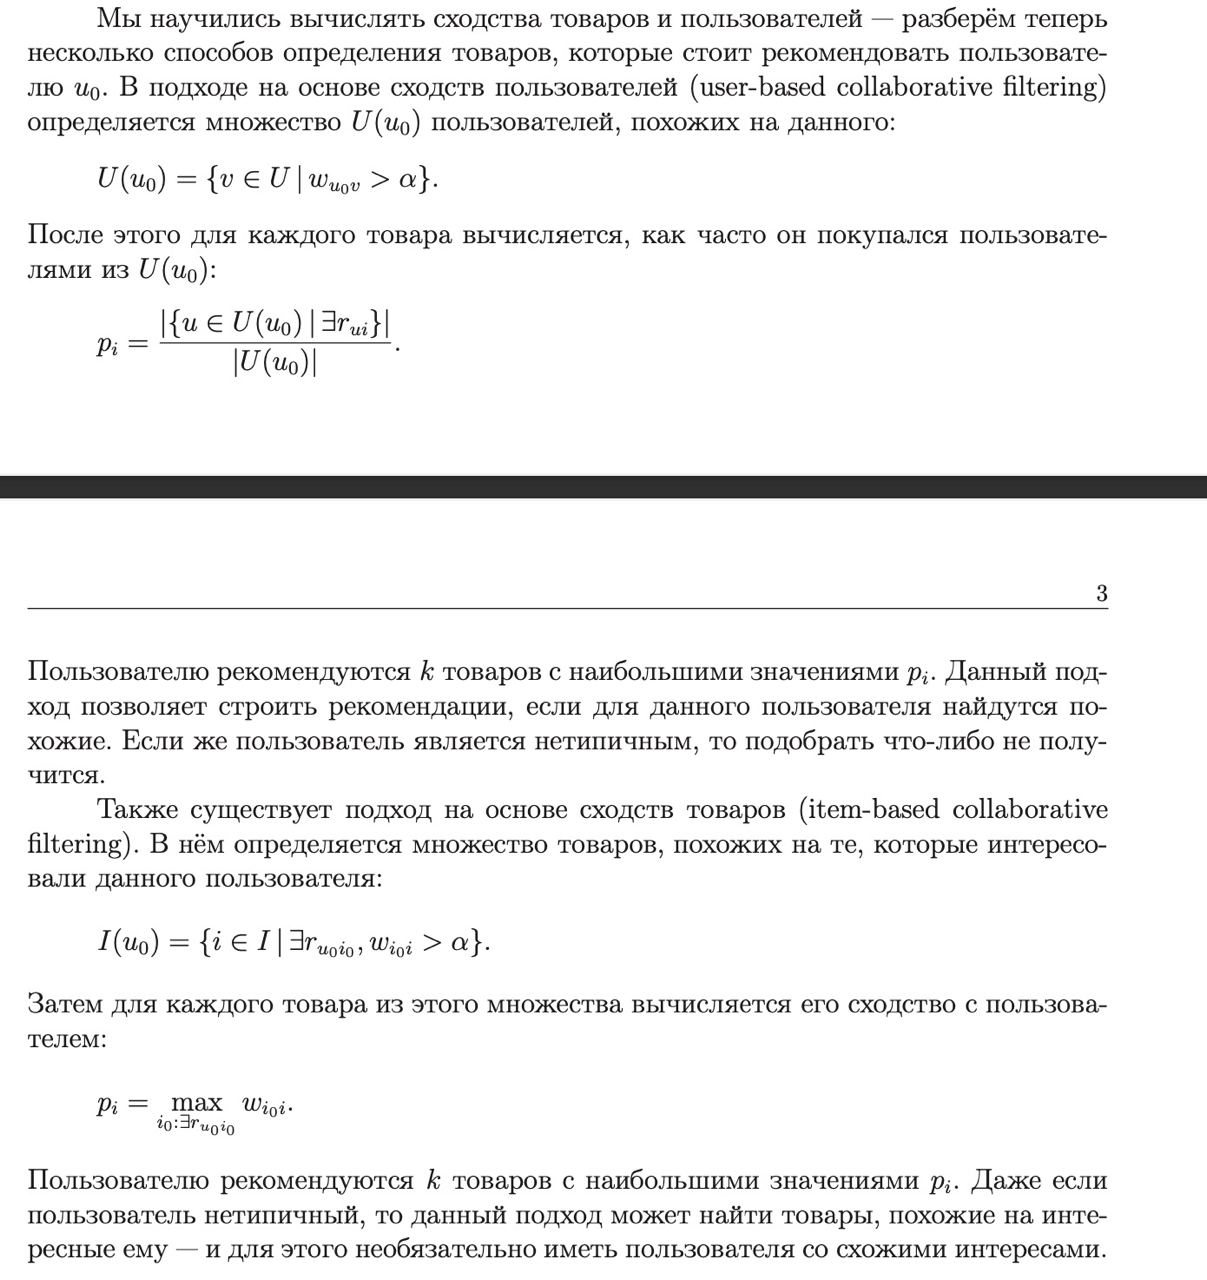
\includegraphics[width=0.7\linewidth]{16_memory2.jpg}
\caption{Конспект Соколова прошлый год}
\label{fig:16_memory2} 
\end{figure}
